\apendice{Descripción de adquisición y tratamiento de datos}
Como se mencionó en la memoria de este proyecto, se han generado datos experimentales propios a partir del sistema de adquisición implementado. No se ha recurrido al uso de bases de datos públicas o registros externos. Para ello, se ha desarrollado un sistema de adquisición personalizado, orientado a la captura de señales fotopletismográficas en distintas condiciones.

\section{Descripción formal de los datos}

Los datos registrados durante el proyecto se almacenan en ficheros CSV, generados automáticamente y en tiempo real por el microcontrolador del sistema a partir de los valores recogidos por el sensor óptico U401-D, gobernado por el chip AFE4490. El proceso de adquisición de los datos fue descrito en la sección de la \textit{Metodología} de la memoria del trabajo.
Cada fichero corresponde a una sesión de adquisición de aproximadamente 30 segundos de duración, con una frecuencia de muestreo cercana a 60 Hz.

El archivo contiene cinco columnas, cuyas variables y rangos observados son:

\begin{itemize}
  \item \textbf{Tiempo (ms)}: Marca temporal de la muestra, iniciando en 0 ms y finalizado el registro en 30 000 ms. Permite reconstruir la señal en el dominio temporal. Los logs tienen esta duración para poder limpiar la señal y tener un rango de valores lo suficientemente extenso como para no perder información y poder analizar los datos de una manera válida.
  
  \item \textbf{IR}: Señal óptica infrarroja medida con el LED de 940 nm encendido. Se utiliza para el análisis de la variabilidad pulsátil del volumen sanguíneo (frecuencia cardíaca) y estimación de SpO\textsubscript{2}. La señal varía cíclicamente con el pulso, reflejando los latidos del corazón.
  
  \item \textbf{AMB\_IR}: Nivel de luz infrarroja ambiente medida con el LED apagado.  Sirve para estimar y corregir la interferencia ambiental en la señal IR. Es útil para eliminar el ruido proveniente de fuentes de luz externas (como luz artificial, luz solar, etc.). Se resta de la señal IR para obtener solo la parte útil emitida por el LED.
  
  \item \textbf{RED}: Señal óptica roja con el LED de 660 nm encendido. La absorción de luz roja varía según el nivel de oxígeno en la sangre. También varía con el pulso, pero de forma distinta a la señal IR.
  
  \item \textbf{AMB\_RED}: Representa la medición de luz roja captada con LED rojo apagado, es decir, la luz ambiental en la misma longitud de onda. Igual que AMB\_IR, se utiliza para corregir la señal RED restando la componente ambiental.

\end{itemize}

\begin{figure}[H]
    \centering
    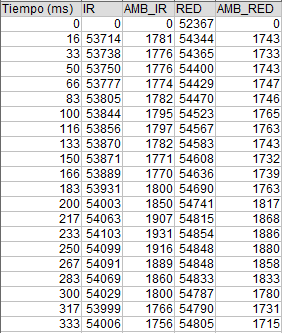
\includegraphics[scale=0.80]{img/Datos crudos csv.png}
    \caption{Ejemplo de unos milisegundos de un registro de datos crudos. \textit{Elaboración propia.}}
    \label{fig:datos_crudos}
\end{figure}

\newpage

Para cada longitud de onda (IR y RED), se realiza:
\begin{itemize}
    \item \texttt{IR\_real = IR - AMB\_IR}
    \item \texttt{RED\_real = RED - AMB\_RED}
\end{itemize}

Esto permite obtener solo la señal útil (emitida por el LED y absorbida por el tejido), eliminando el ruido ambiental. Las señales corregidas se usan luego para detectar picos y calcular el cociente de absorción IR/RED.

\subsection{Rango y unidades de las señales}

Los valores registrados en las columnas \texttt{IR}, \texttt{RED}, \texttt{AMB\_IR} y \texttt{AMB\_RED} no están expresados en unidades físicas como voltios o miliwatios, sino que corresponden a valores crudos digitalizados, generados por el convertidor ADC interno del circuito AFE4490.

Este ADC tiene una resolución de 22 bits con signo, por lo que puede generar un amplio intervalo de valores. Sin embargo, en las configuraciones utilizadas en este proyecto, los valores reales registrados caen dentro de los siguientes rangos típicos:

\begin{itemize}
    \item \textbf{IR}: 30.000 – 65.000 unidades. Señal infrarroja útil, más estable que la roja.
    \item \textbf{RED}: 3.000 – 65.000 unidades. Señal roja, con mayor dispersión entre sesiones.
    \item \textbf{AMB\_IR} y \textbf{AMB\_RED}: 0 – 10.000 unidades. Corresponden a luz ambiental; idealmente deberían ser bajas.
\end{itemize}

Aunque no se cuenta con una calibración para traducir estos valores a magnitudes físicas, su uso es  válido para el análisis de la señal pulsátil y la posterior estimación de parámetros fisiológicos.


\subsection{Análisis de tendencias}

Inicialmente se planteó la hipótesis de que una frecuencia cardíaca más baja estaría asociada a valores medios de señal más altos (por ejemplo, debido a mayor volumen sistólico o perfusión). Sin embargo, el análisis de varios registros no ha mostrado una correlación directa ni consistente entre la frecuencia cardíaca y el valor medio de las señales IR o RED.

Esta variabilidad puede explicarse por múltiples factores, entre ellos:

\begin{itemize}
    \item Diferencias en la presión de colocación del sensor.
    \item Cambios en la perfusión periférica o temperatura de los dedos.
    \item Ruido de fondo e interferencias ópticas del entorno.
    \item Distintas configuraciones del AFE4490 durante las sesiones.
\end{itemize}

Por tanto, el sistema se basa exclusivamente en la relación relativa entre componentes de cada señal y no en su valor absoluto.

\subsection{Alamacenamiento de los datos}

Los archivos se nombran con el formato:

\begin{center}
  \texttt{raw\_data\_\{SpO2\}\_\{HR\}.csv}
\end{center}

donde \texttt{\{SpO2\}} y \texttt{\{HR\}} representan los valores de saturación de oxígeno y frecuencia cardíaca registrados simultáneamente en otro dedo del usuario por un par de pulsioxímetros comerciales externos para validación cruzada. Gracias a la referencia de ambos valores a través del nombre del archivo, se puede validar el valor que se obtiene en la estimación del código.

Los ficheros están clasificados por:

\begin{itemize}
  \item \textbf{Calidad de la señal}: buena o mala.
  \item \textbf{Condición fisiológica del sujeto}: reposo, post-ejercicio, apnea breve, iluminación variable.
\end{itemize}

\section{Descripción clínica de los datos}

Aunque algunos de los conceptos presentados en esta sección ya han sido explicados previamente en el capítulo de fundamentos teóricos, se recogen aquí de forma resumida y aplicada al contexto experimental, de acuerdo con los objetivos específicos de este anexo.


La señal adquirida es una señal PPG, obtenida mediante iluminación del tejido con luz en dos longitudes de onda: infrarrojo (940 nm) y rojo (660 nm). La absorción de la luz depende del contenido de hemoglobina oxigenada y desoxigenada en sangre. La señal resultante tiene dos componentes:

\begin{itemize}
  \item \textbf{Componente DC}: relacionada con tejidos estáticos y sangre no pulsátil.
  \item \textbf{Componente AC}: refleja el pulso arterial y permite detectar la frecuencia cardíaca.
\end{itemize}

Los parámetros fisiológicos que pueden ser extraídos con estos datos son la frecuencia cardíaca y la saturación de oxígeno.

Los datos fueron adquiridos con un sujeto sano adulto bajo diferentes condiciones simuladas:

\begin{itemize}
  \item \textbf{Reposo absoluto}: señal estable, sin interferencias.
  \item \textbf{Post-ejercicio}: incremento de HR y aparición de ruido.
  \item \textbf{Apnea breve}: reducción inducida de SpO\textsubscript{2}.
  \item \textbf{Iluminación variable}: para evaluar la robustez ante interferencia lumínica.
\end{itemize}

Las señales ambientales (\texttt{AMB\_IR} y \texttt{AMB\_RED}) permiten compensar adecuadamente la luz del entorno para mantener la precisión en escenarios reales. Además, se identificaron registros inválidos debido a movimientos, baja perfusión o problemas de contacto, los cuales no fueron eliminados sino clasificados para evaluar el rendimiento del algoritmo en situaciones adversas.

Cuando los datos adquiridos en formato \texttt{.csv} se representan gráficamente en el dominio temporal, se obtiene una señal como la que se muestra a continuación:

\begin{figure}[H]
    \centering
    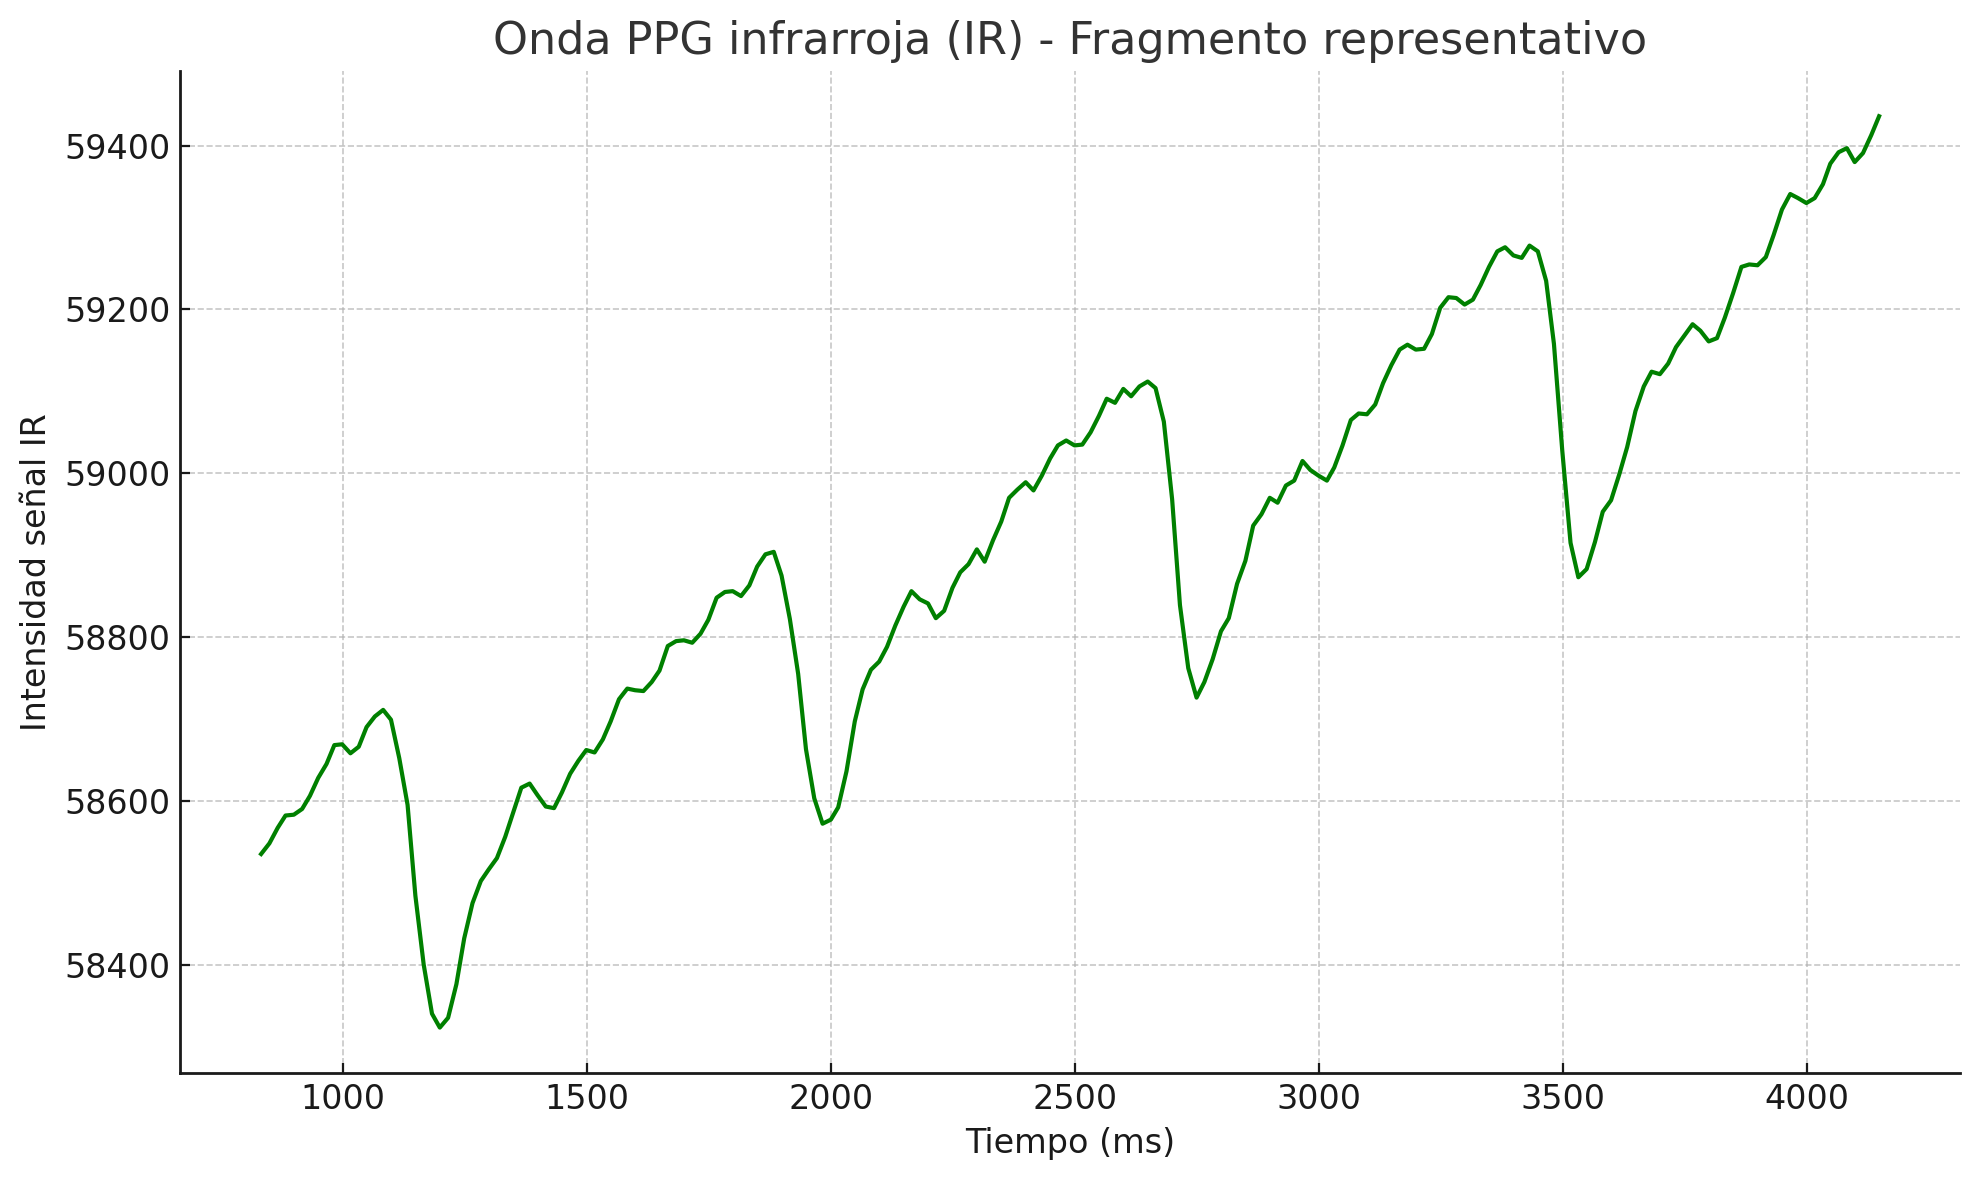
\includegraphics[width=0.95\linewidth]{img/forma_onda_PPG.png}
    \caption{Onda PPG del canal IR. El fragmento muestra aproximadamente 6 pulsos cardíacos completos correspondientes a un registro con HR = 69 bpm. \textit{Elaboración propia.}}
    \label{fig:ppg_morfologia}
\end{figure}

La señal PPG presenta una estructura morfológica característica que refleja directamente los cambios en el volumen sanguíneo arterial. Como se muestra en la Figura~\ref{fig:ppg_partes}, la señal está compuesta por:

\begin{itemize}
    \item \textbf{Pico primario (primary peak)}: punto máximo de cada ciclo, asociado a la presión máxima durante la sístole.
    \item \textbf{Trough}: punto mínimo del ciclo, justo antes del ascenso del siguiente pulso. Se utiliza como referencia para medir la amplitud.
    \item \textbf{Pulse amplitude}: diferencia entre el pico sistólico y el trough. Representa la magnitud del componente pulsátil AC.
    \item \textbf{Pulse width}: duración temporal del ciclo, medida como el tiempo entre dos picos consecutivos. Está relacionada con el intervalo RR y, por tanto, con la frecuencia cardíaca.
    \item \textbf{Pico secundario o muesca dicrota (secondary peak)}: pequeña inflexión o repunte que aparece en la fase de descenso, visible en señales de alta calidad, asociada al cierre de la válvula aórtica.
\end{itemize}

\begin{figure}[H]
    \centering
    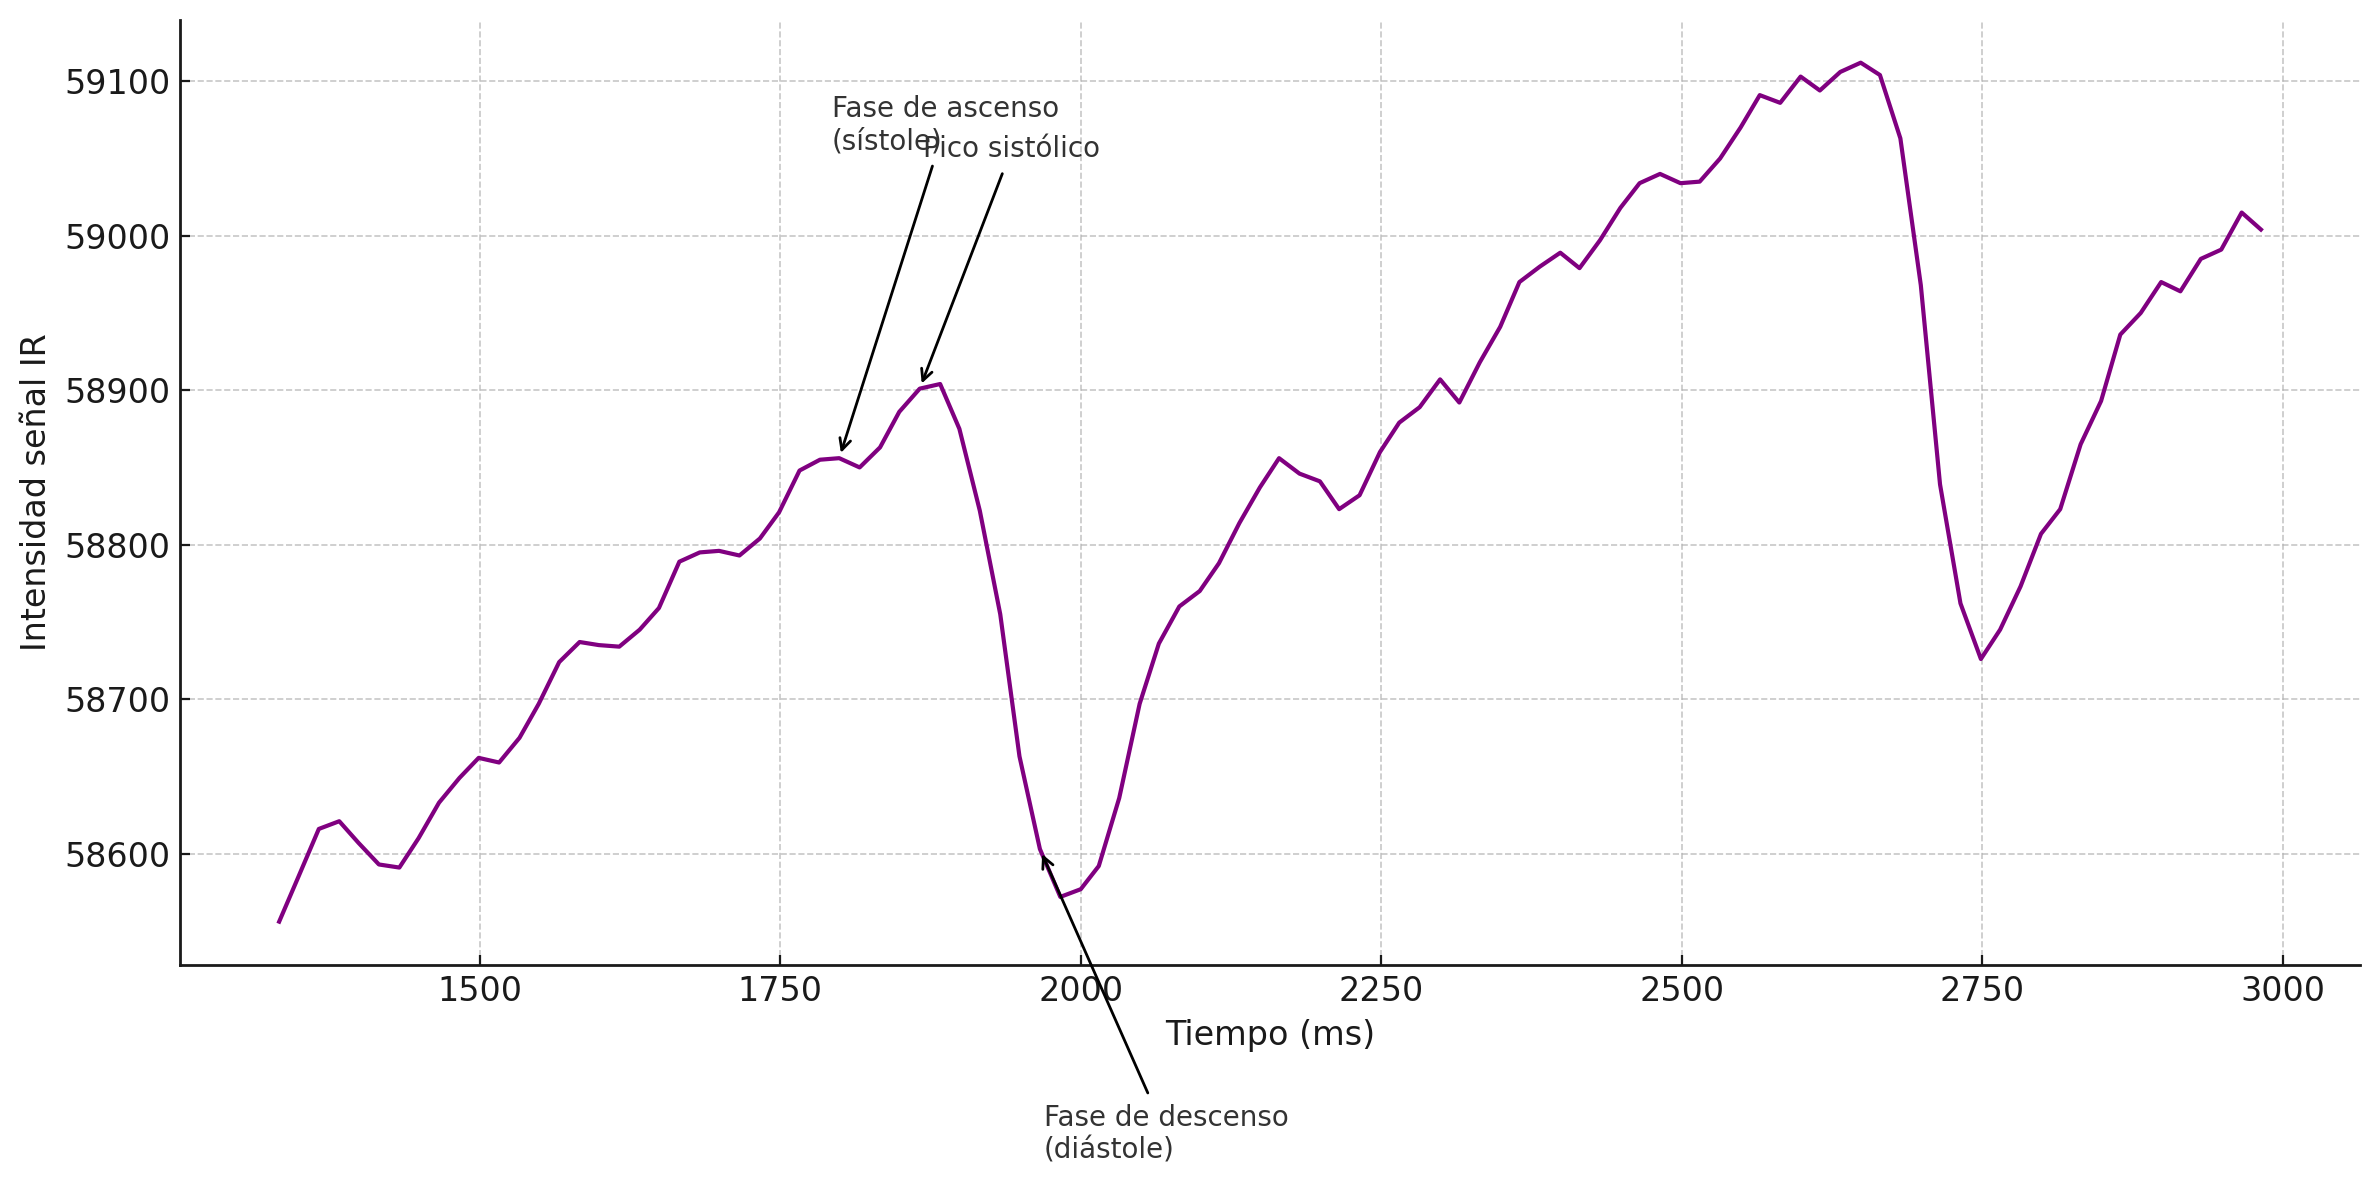
\includegraphics[width=1\linewidth]{img/partesPPG.png}
    \caption{Detalle ampliado de la señal PPG. Se muestran dos pulsos cardíacos completos y se anotan las fases principales de la morfología. Fuente: \cite{oximetria_medium}.}
    \label{fig:ppg_partes}
\end{figure}

Una forma de saber si los datos son válidos para su posterior análisis, es graficar las señales para comprobar que la morfología sea claramente visible y así garantizar una interpretación clínica aceptable. La correcta identificación de los picos es necesaria para el cálculo de la frecuencia cardíaca, y la forma general de la señal (incluyendo su amplitud relativa y periodicidad) afecta directamente a la estimación de la saturación de oxígeno. 

No es indispensable que la señal se comporte de esta manera a lo largo de todo el período que dure la medición, pero sí que es importante que durante unos segundos se mantenga esta estructura para poder identificar los picos necesarios para hacer el cálculo.

El tratamiento posterior de los datos se llevó a cabo en \texttt{Python} mediante entornos de trabajo \texttt{Jupyter Notebook}, donde se aplicaron algoritmos de filtrado digital, detección de picos y cálculo de estimaciones agregadas de SpO\textsubscript{2} y frecuencia cardíaca. Los valores obtenidos se compararon con las medidas externas para evaluar la precisión del sistema.


